\section{Quality evaluation}

The main source of errors in the full pipeline is the \match* step, whose mistakes are then passed on to the \linkDDD* step.
The root cause to the \match* errors is the bubble density.
In fact, if few bubbles are present in the scene, there will be only a handful of candidates near the epiline.
This makes it trivial to choose the correct one, even with basic approaches.
As the bubble density increases, however, the number of candidates close to the epiline augments, too.
With that, the \match* task becomes harder and harder, reaching overwhelming levels also for a human at just 100 bubbles.
With every matching error, the algorithm reconstructs some ``random, isolated bubbles'' that not only are wrong by themselves, but also act as missing points in the trajectory chain, splitting the full trajectory into three separate parts.

% The main errors in the final pipeline are introduced in the \match* step, and then reflected onto the \linkDDD*.
% The main problem of the \match*  is the bubble density in the frames: with few bubbles, the epiline will not provide many candidates, thus making it easier to choose the correct match.
% As the density increases, the presence of more candidates implies more chance for mistakes, which would become ``random, isolated bubbles'' in the 3D view, which also break the trajectories reconstructed by the \link*.

For measuring how good the algorithm behaves with different bubble densities, some synthetic datasets were created in Blender, and used as input for the pipeline.
Such datasets were composed of 30 frames with the same format as the real ones: 960{$\times$}960 images, representing white bubbles over a black background.
The datasets were constructed to have a specific number of bubbles $N$, always visible by all the three cameras observing the scene.
All the bubbles rotate in a clockwise direction, with the same tangential speed: this enables to avoid bubbles shadowing each other, and creates a regular pattern that can be recognized by eye.
Given the specifications of the dataset, ideally the algorithm should be able to reconstruct exactly $N$ 30-frames-long trajectories: more trajectories are index of reconstruction errors.

% For measuring the quality as a function of the number of bubbles, different input datasets were developed in Blender, with the same format as the real data.
% In these datasets, a number $N$ of bubbles rotate in circles around the center of the image, never exiting the field of view of any camera for the full 30 frame duration.
% As such, the algorithm should be ideally able to reconstruct exactly $N$ tracklets with 30 frames of length.

As previously stated, the main source of errors is the \match*.
Errors at this stage position a bubble away from its correct location, splitting its trajectory in three parts.
In particular, for the 30-frames dataset, a single error at frame $f$ would split the full trajectory into two shorter segments, with lengths $f$ and $29-f$, plus a single-frame tracklet, with only the erroneous bubble.
As such, by analyzing the distribution of trajectory lengths, it is possible to evaluate the quality of the reconstruction.

% A single matching error at frame $f$ will move one bubble into the wrong position, splitting the 30-frame trajectory into three, with lengths $f$, $1$ and $29-f$.
% As such, errors can be identified by examining the distribution of trajectory length.

Experiments were conducted with four different datasets, respectively with 50, 100, 250 and 1000 bubbles each.
% In particular, the x-axis contains the trajectory lengths, and the corresponding y-value indicates the percentage of bubbles associated with a trajectory of such length.
% The x-value $x$ will be the percentage value of $N_x{\cdot}x:B$, where $B$ is the total number of bubbles of all frames, and $N_x$ is the number of trajectories with length $x$.
% The $x$ factor is crucial, since it makes the different lengths comparable: without it, the graph would just be the percentage of tracklets with a specific length over the total number of tracklets.
% If that was the case, however, a full trajectory split into 3 pieces would be valued as three times a 
Initially, the graph in figure~\ref{fig:traj-len-distr} was created, with the most intuitive content: the percentage of trajectories with length $x$, for every possible length $x$.
This visualization was however misleading: for example, the 50-bubbles dataset had 29 full-length (30 frames) trajectories, which is more than half.
However, the corresponding point on the graph had a value of about 30\%.
The cause of this inconsistency in the graph is the fact that splitting a theoretical trajectory into smaller ones would increase the total number of trajectories, thus reducing all the percentages.
In other words, the correct reconstruction counts as 1, but a trajectory with an error in the middle counts as 3.
\begin{figure}
	\centerline{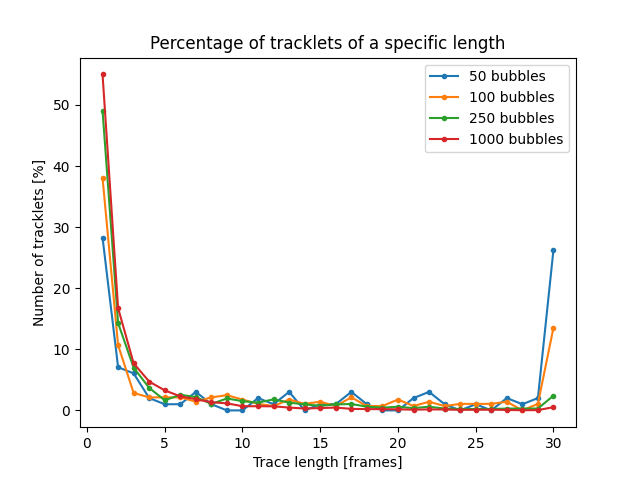
\includegraphics[width=0.7\textwidth]{images/traj-len-graph-first.png}}
	\caption{\centering The distribution of trajectory lengths for the different datasets with varying number of bubbles: considering each trajectory as ``one''}
	\label{fig:traj-len-distr}
\end{figure}

To make up for this error, a new graph was created, depicted in figure~\ref{fig:traj-len-distr-weighted}.
It does not compute the average over the number of trajectories, but over the number of bubbles, which is not affected by the reconstruction quality.
As such, the data points in this new graph are weighted over the trajectory length.
For example, a 1-long trajectory would count as a ``single unit'', while a 30-long trajectory has a value of ``30 units'' for this computation.
This enables to correctly showcase the overall quality of the reconstruction: in the 50-bubbles example considered before, now the value indicated by the graph for complete trajectories is about 60\%, coherent with the measure of 29 fully reconstructed tracklets over the total 50 bubbles.
\begin{figure}
	\centerline{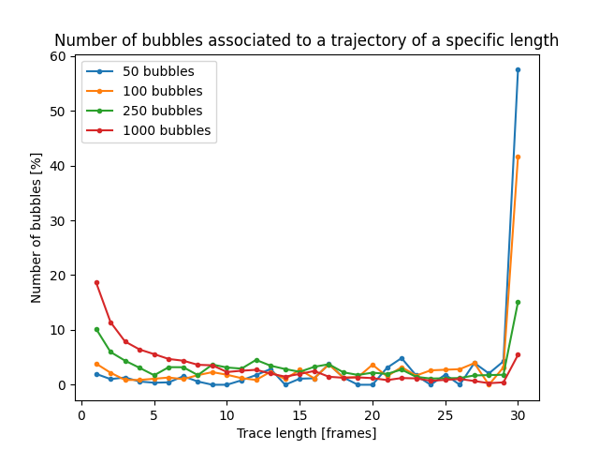
\includegraphics[width=0.7\textwidth]{images/traj-len-graph.png}}
	\caption{\centering The distribution of trajectory lengths for the different datasets with varying number of bubbles: considering trajectories weighted on their length}
	\label{fig:traj-len-distr-weighted}
\end{figure}

In the ideal scenario, both graphs should have a flat value of 0\% for all trajectory lengths, with a 100\% spike at the value 30: whatever departs from this is index of errors.
While it may seem counterintuitive, higher values (not 30) do not necessarily imply better results.
Assume there is a reconstruction error in a tracklet: instead of having a full, 30-frames trajectory, there will be 3, with lengths $f$, $1$ and $29-f$, with $f$ being the wrongly reconstructed frame.
By changing where the mistake was ($f$), the two peaks in the graph will move, spacing from 1 and 29 for $f{=}0$, to 14 and 15 for $f{=}14$.
There would however not be a real effect on the quality of the data: there will always be two coherent tracklets, separated by a missing point.
As such, values smaller than 30 indicate the presence of errors, without correlation between quality and individual lengths.

As visible in figure~\ref{fig:traj-len-distr-weighted}, in the first two datasets most of the tracklets cover the full length, while the quality diminishes visibly with the other datasets.
As such, the quality is considered good with observations of up to 100 bubbles.

% Figure~\ref{fig:traj-len-distr} compares such distribution of lengths for $N$ values of 50, 100, 250, 1000.
% The x axis represents the trajectory length, while the y axis is the percentage of bubbles associated with such length.
% For example, a 30-frames trajectory would count as ``30 units'' in the x=30 bin, while a trajectory split at frame 5 would count as 5 units at x=5, 1 unit at x=1 and 24 units at x=24.
% The percentage is obtained by dividing the value (in ``units'') of each bin by the total value of the graph, which is the total number of detected bubbles.
% Ideally, the graph should have value 0\% for all bins other than 30, which should have a value of 100\%.
% As visible in the graph, a good part of the trajectories is correct up to 100 bubbles, while adding more deteriorates the performance considerably.
% The quality is therefore considered good up to 100 bubbles.
